\documentclass[letterpaper,11pt]{article}
\usepackage[spanish]{babel}
\usepackage[utf8]{inputenc}
\usepackage{graphicx}
\usepackage{amsfonts,amsmath,amssymb,float, amsthm,mathrsfs}  
\usepackage[right=4.5cm,left=2cm,top=3cm,bottom=3cm,headsep= 0.7cm,footskip=0.5cm]{geometry}
\usepackage{enumerate}
\usepackage{wrapfig} 
\usepackage[rflt]{floatflt} 
\usepackage{framed}
%\usepackage[most]{tcolorbox}
\usepackage[dvipsnames]{xcolor}
\colorlet{shadecolor}{green!20}
\setlength\FrameSep{0.5ex}
\usepackage{thmtools}
\usepackage{esint}
\usepackage{cancel}
\usepackage{listings} 
\usepackage{pstricks, caption}
\usepackage[colorlinks]{hyperref}
\usepackage{csquotes}
\usepackage{fullpage}
\usepackage{enumitem}
\usepackage{etoolbox}
\usepackage{tikz}
\usepackage{tikz-3dplot}
\tdplotsetmaincoords{80}{70}
\usetikzlibrary{decorations.markings}
\usetikzlibrary{arrows,babel}
\usepackage[font=small]{caption}
\usepackage{scalerel} %\scaleto{text}{size}
\usepackage{subcaption}
\usepackage{fancyhdr}
\usepackage{comment}
\usepackage{marginnote}
\usepackage{tensor}
\usepackage{cleveref}
\newcommand{\dbar}{\mathchar'26\mkern-12mu d}
\renewcommand*{\marginnotevadjust}{-0.1cm}
\renewcommand*{\marginfont}{\footnotesize}
\setlength{\headheight}{15pt}
\addtolength{\topmargin}{-14.49998pt}
\setlength{\headsep}{15pt}
\setlength{\footskip}{14.49998pt}
\decimalpoint
\newcommand{\grad}{^\circ}
\newlength{\drop}
\DeclareMathOperator{\sign}{sgn}
\DeclareMathOperator{\Log}{Log}
\providecommand{\norm}[1]{\lVert#1\rVert}

\let\cancelorigcolor\CancelColor% Just for conveniency...

\newcommand{\CancelTo}[3][]{%
  \ifblank{#1}{}{%
    \renewcommand{\CancelColor}{#1}%
  }
  \cancelto{#2}{#3}% 
}


\begin{document}

\pagestyle{plain}

\begin{flushleft}\vspace{-2cm}
Departamento de Física \\
Facultad de Cs. Físicas y Matemáticas\\
Universidad de Concepción
\end{flushleft}

\begin{flushright}\vspace{-1.5cm}
\textbf{Tópicos en Relatividad General} 
\end{flushright}



\rule{\linewidth}{0.1mm}

\begin{center}
\textbf{\LARGE Semana 12}
\end{center}

\begin{flushleft}
\textbf{Nombre:} Alejandro Saavedra San Martín. \\
\textbf{Profesor:} Guillermo Rubilar Alegría.
\end{flushleft}

\section{Campos gravitacionales débiles y ondas gravitacionales}

\subsection{Ondas gravitacionales planas: dos polarizaciones}

Consideremos una región sin materia por la que se propaga una onda gravitacional plana de la forma
\begin{equation}
\bar{h}_{\mu\nu} = \Re\left[ A_{\mu\nu} \exp(ik_{\lambda} x^{\lambda})\right], \label{eq:plane-wave-1}
\end{equation}
donde $A_{\mu\nu}$ es el tensor \textbf{amplitud de onda} y $k_{\lambda} = (\omega/c, - k^i)$ es el \textbf{4-vector de onda} \footnote{El tensor $A_{\mu\nu}$ y el vector $k_{\lambda}$ se definen bajo transformaciones de Lorentz.}. Producto de la simetría de la métrica, $A_{\mu\nu}$ es simétrico, entonces son 10 componentes linealmente independientes, constantes y complejas. Si $A_{\mu\nu} = |A_{\mu\nu}| e^{i\varphi_0}$, entonces también podemos escribir
\begin{equation}
\bar{h}_{\mu\nu} = |A_{\mu\nu}| \cos(\omega t - \vec{k} \cdot \vec{x} + \varphi_0). \label{eq:plane-wave-2}
\end{equation}

Introduciendo \eqref{eq:plane-wave-1} en la ecuación de onda homogénea, $\square \bar{h}_{\mu\nu} = 0$, obtenemos que
\begin{align}
\square\left( 
A_{\mu\nu} e^{ik_{\lambda} k^{\lambda}}\right) &= 0, \\
A_{\mu\nu} \eta^{\alpha\beta} \partial_{\alpha} \partial_{\beta} \left( 
 e^{ik_{\lambda} k^{\lambda}}\right) &= 0, \\
A_{\mu\nu} \eta^{\alpha\beta} \partial_{\alpha} \left( 
 e^{ik_{\lambda} k^{\lambda}} \partial_{\beta}(k_{\rho} x^{\rho})\right) &= 0, \\
A_{\mu\nu} \eta^{\alpha\beta} \partial_{\alpha} \left( 
 e^{ik_{\lambda} k^{\lambda}} k_{\rho} \delta_{\beta}^{\rho}\right) &= 0,\\
 A_{\mu\nu} e^{ik_{\lambda} k^{\lambda}} \eta^{\alpha\beta} k_{\beta} \partial_{\alpha} (k_{\rho} x^{\rho}) &= 0, \\
\bar{h}_{\mu\nu} \eta^{\alpha\beta} k_{\beta} k_{\rho} \delta_{\alpha}^{\rho} &= 0, \\
\bar{h}_{\mu\nu} \eta^{\alpha\beta} k_{\beta} k_{\alpha} &= 0, \\
\bar{h}_{\mu\nu} k^{\beta} k_{\beta} &= 0.
\end{align}

Como queremos soluciones no triviales, encontramos que
\begin{shaded}
\begin{equation}
k_{\lambda} k^{\lambda} = 0. \label{eq:plane-wave-3}
\end{equation}
\end{shaded}

Por otro lado, de la condición del gauge de Lorenz, 
\begin{align}
\partial^{\nu} \bar{h}_{\mu\nu} &= 0, \\
\eta^{\nu\alpha}\partial_{\alpha} \left(A_{\mu\nu} e^{ik_{\lambda} x^{\lambda}} \right) &= 0, \\
A_{\mu\nu} e^{ik_{\lambda} x^{\lambda}} \eta^{\nu\alpha} \partial_{\alpha}(k_{\rho} x^{\rho}) &= 0, \\
A_{\mu\nu} e^{ik_{\lambda} x^{\lambda}} \eta^{\nu\alpha} k_{\rho} \delta_{\alpha}^{\rho} &= 0, \\
A_{\mu\nu} e^{ik_{\lambda} x^{\lambda}} \eta^{\nu\alpha} k_{\alpha} &= 0,\\
A_{\mu\nu} e^{ik_{\lambda} x^{\lambda}} k^{\nu} &= 0.
\end{align}

Así, otra condición que debe cumplir el ansatz \eqref{eq:plane-wave-1} es
\begin{shaded}
\begin{equation}
A_{\mu\nu} k^{\nu} = 0. \label{eq:plane-wave-4}
\end{equation}
\end{shaded}

Estas últimas cuatro condiciones reducen el número de componentes linealmente independientes de la amplitud $A_{\mu\nu}$ de 10 a 6. Adicionalmente, podemos usar la libertad de gauge residual para reducir el número de componentes independientes a sólo 2.

En efecto, dado un vector tipo luz $k_{\mu}$ arbitrario, podemos elegir los ejes coordenados (por medio de una transformación de Lorentz) de modo que la onda se propague a lo largo del eje $z$ arbitrario, es decir, tal que
\begin{equation}
k^{\mu} = \left( \frac{\omega}{c},0,0,k\right), \qquad k_{\mu} = \left( \frac{\omega}{c},0,0,-k\right), \label{eq:plane-wave-5}
\end{equation}
con $k > 0$. Si usamos la condición \eqref{eq:plane-wave-3}, tenemos que
\begin{equation}
k^{\mu} k_{\mu} = (k^0)^2 - (k^1)^2 - (k^2)^2 - (k^3)^2 = \frac{\omega^2}{c^2} - k^2 = 0,
\end{equation}
es decir, $\omega/c = k$. Luego, las ecuaciones en \eqref{eq:plane-wave-5} nos quedan
\begin{equation}
k^{\mu} = \left(k,0,0,k\right), \qquad k_{\mu} = \left(k,0,0,-k\right). \label{eq:plane-wave-6}
\end{equation}

Por otro lado, la condición \eqref{eq:plane-wave-4} nos dice que
\begin{align}
k^{\mu} A_{\mu\nu} &= 0, \\
k^0 A_{0\nu} + k^1 A_{1\nu} + k^2 A_{2\nu} + k^3 A_{3\nu} &= 0, \\
k  A_{0\nu} + k A_{3\nu} &= 0, \\
A_{0\nu} &= - A_{3\nu}, \qquad \nu = 0,1,2,3. \label{eq:plane-wave-7}
\end{align}

Usando la métrica de Minkowski, escribamos el tensor de amplitud de onda con todos sus índices contravariantes: 
\begin{equation}
A^{\mu\nu} = \eta^{\mu\rho} \eta^{\nu\sigma} A_{\rho\sigma}.
\end{equation}

Entonces, podemos escribir
\begin{align}
A^{00} &= \eta^{0\rho} \eta^{0\sigma} A_{\rho\sigma} = A_{00}, \\
A^{0i} &= \eta^{0\rho} \eta^{i\sigma} A_{\rho\sigma} = - A_{0i}, \\
A^{30} &= \eta^{3\rho} \eta^{0\sigma} A_{\rho\sigma} = - A_{30}, \\
A^{3i} &= \eta^{3\rho} \eta^{i\sigma} A_{\rho\sigma} = A_{3i},
\end{align}
donde $i = 1,2,3$. Así, la condición \eqref{eq:plane-wave-7} puede escribirse como
\begin{equation}
A^{00} = A^{30}, \qquad A^{0i} = A^{3i}. 
\end{equation}

Explicitando las componentes espaciales, obtenemos que
\begin{align}
A^{00} &= A^{30}, \\
A^{01} &= A^{31}, \\
A^{02} &= A^{32}, \\
A^{03} &= A^{33}. \\
\end{align}

Como $A^{\mu\nu}$ es un tensor simétrico, 
\begin{align}
A^{00} &= A^{30} = A^{03} = A^{33}, \label{eq:plane-wave-8} \\
A^{01} &= A^{10} = A^{31} = A^{13}, \label{eq:plane-wave-9}\\
A^{02} &= A^{20} = A^{32} = A^{23}.\label{eq:plane-wave-10}
\end{align}

Si representamos $A_{\mu\nu}$ como una matriz y usamos las ecuaciones \eqref{eq:plane-wave-8}-\eqref{eq:plane-wave-10}, podemos escribir
\begin{equation}
A^{\mu\nu} = \begin{pmatrix}
A^{00} & A^{01} & A^{02} & A^{00} \\
A^{01} & A^{11} & A^{12} & A^{01} \\
A^{02} & A^{12} & A^{22} & A^{02} \\
A^{00} & A^{01} & A^{02} & A^{00} 
\end{pmatrix} = \begin{pmatrix}
A^{33} & A^{13} & A^{23} & A^{33} \\
A^{13} & A^{11} & A^{12} & A^{13} \\
A^{23} & A^{12} & A^{22} & A^{23} \\
A^{33} & A^{13} & A^{23} & A^{33} 
\end{pmatrix}. \label{eq:plane-wave-11}
\end{equation}

Consideremos ahora la transformaión de gauge definida por
\begin{equation}
\xi^{\mu} = - \Re\left[i \epsilon^{\mu} \exp(i k_{\lambda} x^{\lambda}) \right], \label{eq:plane-wave-12}
\end{equation}
donde $\epsilon^{\mu}$ son constantes, que ajustaremos a continuación. Esta elección de $\xi^{\mu}$ satisface $\square \xi^{\mu} = 0$, pues tiene la forma de una onda plana, de modo que la transformación preserva la condición del gauge de Lorenz.  
Del documento de la semana 11 probamos que al realizar la transformación de gauge, la nueva perturbación $h_{\mu\nu}^{'(1)}$ tiene la forma
\begin{equation}
h_{\mu\nu}^{'(1)} = h_{\mu\nu}^{(1)} - \partial_{\mu} \xi_{\nu}^{(1)} - \partial_{\nu} \xi_{\mu}^{(1)}. \label{eq:plane-wave-13}
\end{equation}

Como
\begin{equation}
\bar{h}_{\mu\nu} := h_{\mu\nu} - \frac{1}{2} \eta_{\mu\nu}h,
\end{equation}
al hacer la transformación de gauge, tenemos que
\begin{align}
\bar{h}_{\mu\nu}' &= h_{\mu\nu}' - \frac{1}{2} \eta_{\mu\nu}h' \nonumber  \\
&=  h_{\mu\nu} - \partial_{\mu} \xi_{\nu} - \partial_{\nu} \xi_{\mu} - \frac{1}{2}\eta_{\mu\nu} \eta^{\rho\sigma} h_{\rho\sigma}' \nonumber \\
&= h_{\mu\nu} - \partial_{\mu} \xi_{\nu} - \partial_{\nu} \xi_{\mu} - \frac{1}{2}\eta_{\mu\nu} \eta^{\rho\sigma} \left(  h_{\rho\sigma} - \partial_{\rho} \xi_{\sigma} - \partial_{\sigma} \xi_{\rho} \right) \nonumber \\
&= \left(h_{\mu\nu} - \frac{1}{2} \eta_{\mu\nu} h \right)  - \partial_{\mu} \xi_{\nu} - \partial_{\nu} \xi_{\mu} + \eta_{\mu\nu} \partial_{\rho} \xi^{\rho} \nonumber \\
&= \bar{h}_{\mu\nu} - \eta_{\nu\alpha} \partial_{\mu} \xi^{\alpha} - \eta_{\mu\alpha} \partial_{\nu} \xi^{\alpha} +  \eta_{\mu\nu} \partial_{\rho} \xi^{\rho}.
\end{align}

Reemplazando \eqref{eq:plane-wave-1} y \eqref{eq:plane-wave-12} en \eqref{eq:plane-wave-13}, podemos escribir
\begin{align}
\bar{h}_{\mu\nu}' &=  \bar{h}_{\mu\nu} - \eta_{\nu\alpha} \partial_{\mu} \xi^{\alpha} - \eta_{\mu\alpha} \partial_{\nu} \xi^{\alpha} +  \eta_{\mu\nu} \partial_{\rho} \xi^{\rho} \nonumber \\
&=\Re\left\{ A_{\mu\nu} \exp(ik_{\lambda} x^{\lambda}) + \eta_{\nu\alpha} \partial_{\mu}\left( i \epsilon^{\alpha} \exp(i k_{\lambda} x^{\lambda}) \right) + \eta_{\mu\alpha}  \partial_{\nu}\left( i \epsilon^{\alpha} \exp(i k_{\lambda} x^{\lambda})\right) - \eta_{\mu\nu} \partial_{\rho} \left( i \epsilon^{\rho} \exp(i k_{\lambda} x^{\lambda}) \right) \right\} \nonumber \\
&= \Re\left\{\left[A_{\mu\nu} + i \eta_{\nu\alpha} \epsilon^{\alpha} \partial_{\mu}\left( i k_{\rho} x^{\rho} \right) + i \eta_{\mu\alpha} \epsilon^{\alpha} \partial_{\nu}\left(i k_{\rho} x^{\rho} \right)  - \eta_{\mu\nu} i \epsilon^{\rho} \partial_{\rho}\left(i k_{\sigma}x^{\sigma}\right)\right]\exp(ik_{\lambda} x^{\lambda})  \right\} \nonumber \\
&= \Re\left\{\left[A_{\mu\nu} - \eta_{\nu\alpha} \epsilon^{\alpha} k_{\mu} - \eta_{\mu\alpha} \epsilon^{\alpha} k_{\nu} + \eta_{\mu\nu}  \epsilon^{\rho} k_{\rho}\right]\exp(ik_{\lambda} x^{\lambda})  \right\} \nonumber \\
&= \Re\left\{\left[A_{\mu\nu} - \epsilon_{\nu} k_{\mu} - \epsilon_{\mu} k_{\nu} + \eta_{\mu\nu}  \epsilon^{\rho} k_{\rho}\right]\exp(ik_{\lambda} x^{\lambda})  \right\}.
\end{align}

Por lo tanto, la nueva perturbación $\bar{h}_{\mu\nu}'$ tiene la misma forma de una onda plana monocromática pero con nueva amplitud
\begin{equation}
A'_{\mu\nu} = A_{\mu\nu} - \epsilon_{\mu} k_{\nu} - \epsilon_{\nu} k_{\mu} + \eta_{\mu\nu} (\epsilon^{\rho} k_{\rho}). \label{eq:plane-wave-14}
\end{equation}

Usando \eqref{eq:plane-wave-6} y \eqref{eq:plane-wave-11} podemos escribir la transformación \eqref{eq:plane-wave-14} explícitamente como
\begin{align}
A'^{00} &= A^{00} - \epsilon^{0} k^{0} - \epsilon^{0} k^{0} + \eta^{00} (\epsilon^{\rho} k_{\rho}) \nonumber \\
&= A^{00} - 2 \epsilon^{0} k  + (\epsilon^{0} k - \epsilon^{3} k) \nonumber \\
&= A^{00} - k (\epsilon^0 + \epsilon^3), \\
A'^{01} &= A^{01} - \epsilon^{0} k^{1} - \epsilon^{1} k^{0} + \eta^{01} (\epsilon^{\rho} k_{\rho}) \nonumber \\
&= A^{01} - k \epsilon^1, \\
A'^{02} &= A^{02} - \epsilon^{0} k^{2} - \epsilon^{2} k^{0} + \eta^{02} (\epsilon^{\rho} k_{\rho}) \nonumber \\
&= A^{02} - k \epsilon^2, \\
A'^{11} &= A^{11} - \epsilon^{1} k^{1} - \epsilon^{1} k^{1} + \eta^{11} (\epsilon^{\rho} k_{\rho}) \nonumber \\
&= A^{11} - k(\epsilon^0 - \epsilon^3), \\
A'^{12} &= A^{12} - \epsilon^{1} k^{2} - \epsilon^{2} k^{1} + \eta^{12} (\epsilon^{\rho} k_{\rho}) \nonumber \\
&= A^{12}, \\
A'^{22} &= A^{22} - \epsilon^{2} k^{2} - \epsilon^{2} k^{2} + \eta^{22} (\epsilon^{\rho} k_{\rho}) \nonumber \\
&= A^{22} - k(\epsilon^0 - \epsilon^3).
\end{align}

Podemos entonces elegir las constantes $\epsilon^{\mu}$ de modo que la amplitud $A^{'\mu\nu}$ adopte una forma simple. En particular, resulta conveniente imponer que 
\begin{equation}
A^{'00} \stackrel{!}{=} A^{'01} \stackrel{!}{=} A^{'02} \stackrel{!}{=} 0,\qquad A^{'11} \stackrel{!}{=} - A^{'22}.
\end{equation}

Encontremos los $\epsilon^{\mu}$ que se requiere elegir para llegar a esta elección particular de $A^{'\mu\nu}$. Para ello, debemos resolver el siguiente sistema de ecuaciones para las incógnitas $\epsilon^{\mu}$:
\begin{align}
A^{00} - k(\epsilon^0 + \epsilon^3) &= 0, \label{eq:plane-wave-15}\\
A^{01} - k \epsilon^1 &= 0, \label{eq:plane-wave-16}\\
A^{02} - k\epsilon^2 &= 0, \label{eq:plane-wave-17}\\
A^{11} - k(\epsilon^0 - \epsilon^3) &= - A^{22} + k (\epsilon^0 - \epsilon^3). \label{eq:plane-wave-18}
\end{align}

Usando las ecuaciones \eqref{eq:plane-wave-16} y \eqref{eq:plane-wave-17}, es directo ver que
\begin{align}
\epsilon^1 &= \frac{A^{01}}{k}, \label{eq:epsilon-1}\\
\epsilon^2 &= \frac{A^{02}}{k}. \label{eq:epsilon-2}
\end{align}

Reescribamos las ecuaciones \eqref{eq:plane-wave-15} y \eqref{eq:plane-wave-18}, respectivamente, de la siguiente forma:
\begin{align}
2 A^{00} &= 2k(\epsilon^0 - \epsilon^3), \label{eq:plane-wave-19}\\
A^{11} + A^{33} &= 2k(\epsilon^0 - \epsilon^3). \label{eq:plane-wave-20}
\end{align}

Si sumamos y restamos las ecuaciones \eqref{eq:plane-wave-19} y \eqref{eq:plane-wave-20}, obtenemos las componentes faltante de $\xi^{\mu}$:
\begin{align}
\epsilon^0 &= \frac{1}{4k} \left( 2A^{00} + A^{11} + A^{22}\right), \label{eq:epsilon-3} \\
\epsilon^3 &= \frac{1}{4k} \left( 2A^{00} - A^{11} - A^{22}\right). \label{eq:epsilon-4}
\end{align}

Por lo tanto, bajo la transformación de gauge \eqref{eq:plane-wave-12} con $\epsilon^{\mu}$ dados por las ecuaciones \eqref{eq:epsilon-1}, \eqref{eq:epsilon-2}, \eqref{eq:epsilon-3} y \eqref{eq:epsilon-4}, la nueva amplitud puede escribirse, en representación matricial, como
\begin{equation}
A^{'\mu\nu} = \begin{pmatrix}
0 & 0 & 0 & 0 \\
0 & A^{'11} & A^{'12} & 0 \\
0 & A^{'12} & -A^{'11} & 0 \\
0 & 0 & 0 & 0 
\end{pmatrix} = A^{'11} \begin{pmatrix}
0 & 0 & 0 & 0 \\
0 & 1 & 0 & 0 \\
0 & 0 & -1 & 0 \\
0 & 0 & 0 & 0 
\end{pmatrix} + A^{'12} \begin{pmatrix}
0 & 0 & 0 & 0 \\
0 & 0 & 1 & 0 \\
0 & 1 & 0 & 0 \\
0 & 0 & 0 & 0 
\end{pmatrix} .
\end{equation}

Debido a esta elección de gauge se satisface $A_{\mu}^{'\mu} = 0$, entonces $\bar{h}' = h' = 0$, es decir, la perturbación es de traza nula y $h'_{\mu 0} = h'_{\mu 3}$. Por estas razones, $A^{'\mu\nu}$ describe una solución en el \textbf{gauge transversal sin traza} (TT). En este sentido, una onda gravitacional plana es \textit{transversal} y tiene sólo 2 \textit{estados de polarización independientes}. 

Si escribimos las amplitudes complejas $A^{'11}$ y $A^{'12}$ en su forma polar:
\begin{equation}
A^{'11} =: h_{+} e^{-i\varphi_{+}}, \qquad A^{'12} =: h_{\times} e^{-i\varphi_{\times}},
\end{equation}
las perturbaciones $h'_{\mu\nu}$ a primer orden de la métrica no nulas son:
\begin{align}
h'_{11} &= - h'_{22} = \Re\left[ h_{+} e^{-i\varphi_{+}} e^{ik_{\mu} x^{\mu}} \right] = h_{+} \cos(\omega t - \vec{k} \cdot \vec{x} - \varphi_{+}), \label{eq:plane-wave-21}\\
h'_{12} &= h'_{21} = \Re\left[ h_{\times} e^{-i\varphi_{\times}} e^{ik_{\mu} x^{\mu}} \right] = h_{x} \cos(\omega t - \vec{k} \cdot \vec{x} - \varphi_{\times}).\label{eq:plane-wave-22}
\end{align} 

Por lo tanto, el elemento de línea correspondiente a una onda gravitacional propagándose a lo largo del eje $z$ positivo, con vector de  onda $k$ y frecuencia $\omega = ck$, con amplitudes $h_{+}$ y $h_{\times}$, y fases $\varphi_{+}$ y $\varphi_{\times}$ respectivamente, es dado por 
\begin{align}
ds^2 &= g_{\mu\nu} dx^{\mu} dx^{\nu} \nonumber \\
&= \left(\eta_{\mu\nu} + h_{\mu\nu}' \right) dx^{\mu} dx^{\nu} \nonumber \\
&= \eta_{\mu\nu} dx^{\mu} dx^{\nu} +  h_{11}' dx^{1}dx^{1} + h_{22}' dx^{2}dx^{2} + h_{12}' dx^{1} dx^{2} + h_{21}' dx^{2} dx^{1}.
\end{align}

Reemplazando \eqref{eq:plane-wave-21} y \eqref{eq:plane-wave-22}, podemos escribir
\begin{shaded}
\begin{equation}
ds^2 = c^2dt^2 - d\vec{x}^2 + h_{+}\cos(\omega t - kz - \varphi_{+})(dx^2 - dy^2) + 2h_{\times} \cos(\omega t - kz - \varphi_{\times}) dxdy. \label{eq:plane-wave-23}
\end{equation}
\end{shaded}

Consideremos por separado las dos posbiles polarizaciones linealmente independientes de la onda gravitacional plana. Para el primer estado de polarización posible, con $h_{+} \neq 0$ y $h_{\times} = 0$, tendremos que el elemento de línea se reduce a
\begin{equation}
ds^2 = c^2dt^2 - d\vec{x}^2 + h_{+}\cos(\omega t - kz - \varphi_{+})(dx^2 - dy^2). \label{eq:plane-wave-24}
\end{equation}

En cambio, para el segundo estado de polarización independiente, con $h_{+} = 0$ y $h_{\times} \neq 0$,
\begin{equation}
ds^2 = c^2dt^2 - d\vec{x}^2 + 2h_{\times} \cos(\omega t - kz - \varphi_{\times}) dxdy. \label{eq:plane-wave-25}
\end{equation}

Ahora, tomemos el elemento de línea \eqref{eq:plane-wave-24} correspondiente al primer estado de polarización y efectuemos una rotación de los ejes coordenados en un ángulo de $45$ grados en torno al eje de propagación de la onda. Es decir, indroduzcamos el nuevo sistema coordenado $x^{'\mu} = (ct,x',y',z')$, con \footnote{En general, cualquier rotación en el plano $xy$ en un ángulo $\theta$ en torno al eje $z$, transforma $(x,y) \rightarrow (x',y')$, con $x' = x \cos \theta + y \sin\theta$ e $y' = - x \sin\theta + y \cos \theta$.}
\begin{align}
x' &=  x \cos\left(\frac{\pi}{4}\right) + y \sin\left(\frac{\pi}{4}\right) = \frac{1}{\sqrt{2}}(x + y), \\
y' &= - x \sin\left(\frac{\pi}{4}\right) + y \cos \left(\frac{\pi}{4}\right) = -\frac{1}{\sqrt{2}}(x- y).
\end{align}

La transformación inversa esta dada por
\begin{align}
x &=  x' \cos\left(-\frac{\pi}{4}\right) + y' \sin\left(-\frac{\pi}{4}\right) = \frac{1}{\sqrt{2}}(x' - y'), \\
y &= - x' \sin\left(-\frac{\pi}{4}\right) + y' \cos \left(-\frac{\pi}{4}\right) = \frac{1}{\sqrt{2}}(x' + y').
\end{align}

Así, el elemento de línea \eqref{eq:plane-wave-24} puede escribir, en estas nuevas coordenadas, como
\begin{align}
ds^2 &= c^2 dt^2 - d\vec{x}\,'^2 + h_{+} \cos(kz - \varphi_{+})\left[\frac{1}{2}(dx' - dy')^2 - \frac{1}{2} (dx' + dy')^2\right] \nonumber \\
&= c^2 dt^2 - d\vec{x}\,'^2 + h_{+} \cos(kz - \varphi_{+})\left[\frac{1}{2}(dx'^2 - 2 dx'dy' + dy'^2) - \frac{1}{2} (dx'^2 + 2dx'dy' + dy'^2)\right] \nonumber \\
&= c^2 dt^2 - d\vec{x}\,'^2 - 2 h_{+} \cos(kz - \varphi_{+})dx'dy'.
\end{align}

Concluimos de este modo que los elementos de línea de las ondas gravitacionales planas correspondientes a los dos estados de polarizacióm físicos, y por consiguiente sus efectos, difieren
(obviando su amplitud y fases eventualmente diferentes) sólo en una rotación de $\pi/4$ en el plano normal a la propagación de la onda. Por lo tanto, podemos restringir nuestro estudio a sólo un estado de polarización en particular.

\subsection{Efectos de una onda gravitacional: principio de un detector de ondas gravitacionales}

Consideremos una región del espaciotiempo por donde viaja una onda gravitacional plana, con vector de onda $k^{\mu} = (k,0,0,k)$ ($k > 0$) dado.  Del documento de la semana 10, encontramos que, a primer orden,
\begin{equation}
\Gamma^{\lambda}_{(1)\mu\nu} = \frac{1}{2} \eta^{\lambda\rho} \left(\partial_{\mu} h_{\nu\rho}^{(1)} + \partial_{\nu} h_{\mu\rho}^{(1)} - \partial_{\rho} h_{\mu\nu}^{(1)} \right). \label{eq:GW-effects-1}
\end{equation}

En en el gauge TT, $h_{0\mu} = h_{\mu 0} = 0$ y $h_{3\mu} = h_{\mu 3} = 0$, entonces, a primer orden,
\begin{equation}
\Gamma^{\lambda}_{00} = \frac{1}{2} \eta^{\lambda\rho} \left(\cancelto{0}{\partial_{0} h_{0\rho}^{(1)}} + \cancelto{0}{\partial_{0} h_{0\rho}^{(1)}} - \cancelto{0}{\partial_{\rho} h_{00}^{(1)}} \right) = 0. \label{eq:GW-effects-2}
\end{equation}

Consideremos la ecuación de la geodésica (tipo tiempo)
\begin{equation}
\frac{d^2x^{\mu}}{d\tau^2} + \Gamma^{\mu}_{\nu\lambda} \frac{dx^{\nu}}{d\tau} \frac{dx^{\lambda}}{d\tau} = 0. \label{eq:GW-effects-3}
\end{equation} 

Usando \eqref{eq:GW-effects-2}, tenemos que las curvas tipo tiempo dadas por $x^{\mu}(\tau) = (c\tau,\vec{x}_0)$, con $\vec{x}_0$ constante son geodésicas. En efecto,
\begin{align}
\frac{d^2x^{\mu}}{d\tau^2} + \Gamma^{\mu}_{\nu\lambda} \frac{dx^{\nu}}{d\tau} \frac{dx^{\lambda}}{d\tau} &= 0 + \Gamma^{\mu}_{00} \left(\frac{dx^0}{d\tau}\right)^2 +  2 \Gamma^{\mu}_{0i} \frac{dx^0}{d\tau} \cancelto{0}{\frac{dx^i}{d\tau}} + \Gamma^{\mu}_{ij} \cancelto{0}{\frac{dx^i}{d\tau} \frac{dx^j}{d\tau}} \nonumber\\
&= \Gamma^{\mu}_{00} c^2 \nonumber\\ 
&= 0.
\end{align}

Ésto implica que una partícula de prueba ubicada en $\vec{x} = \vec{x}_0$ e inicialmente en reposo respecto al sistema coordenado (SC) cuasi-inercial, es decir, con $(d\vec{x}/dt)(0) = \vec{0}$, permanecerá con sus coordenadas espaciales constante en el futuro. Esto no implica, sin embargo, que la ``distancia" (o, más precisamente, el tiempo de vuelo) entre distintos cuerpos de prueba inicialmente en reposo en el SC usado sea constante, ya que la métrica del espaciotiempo varía tanto en el espacio como en el tiempo. En otras palabras, el efecto de una onda gravitacional se anula si hay sólo una partícula, pues, por el principio de equivalencia fuerte, existe un sistema de referencia localmente inercial. Entonces, es necesario más de una partícula para detectar un efecto de estas ondas gravitacionales, por ejemplo, considerar dos partículas de masas $m$ ubicadas en el plano $xy$ con  una onda gravitacional plana que viaja en dirección del eje $z$, ver figura \ref{fig:Efecto-GW-1}. La ``distancia" será proporcional al tiempo de vuelo de un fotón que es emitido en $x^{\mu}_{\text{i}} = (0,\vec{0})$, recibido en el evento $x^{\mu}_{\text{r}_1} = (ct_{\text{r}_1},\vec{x}_0)$ y reflejado hacia el evento $x^{\mu}_{\text{r}_2} = (ct_{\text{r}_2},\vec{0})$, ver figura \ref{fig:Efecto-GW-2}.


\begin{figure}
    \centering
    \begin{subfigure}[t]{0.48\textwidth}
        \centering
        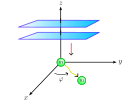
\includegraphics[width=\linewidth]{Efecto-GW-1}
        \caption{Dos partículas de masas $m$ ubicadas en el plano $xy$ con una onda gravitacional plana (planos azules) incidente que viaja en dirección $z$. El tiempo de vuelo se mide con el haz de luz en amarillo.}
        \label{fig:Efecto-GW-1}
    \end{subfigure}\hskip 1em%
    \begin{subfigure}[t]{0.39\textwidth}
        \centering
        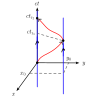
\includegraphics[width=\linewidth]{Efecto-GW-2}
        \caption{Diagrama del espaciotiempo (substrayendo la coordenada espacial $z$) de las dos masas $m$, donde se lanza una haz de luz para medir el tiempo de vuelo (curva roja).}
        \label{fig:Efecto-GW-2}
    \end{subfigure}
\end{figure}

El cálculo que se hará a continuación considera un conjunto de partículas de prueba ubicadas inicialmente en un círculo en el plano $xy$, de radio $R$ en coordenadas cuasi-inerciales, y el movimiento de ida y regreso de fotones desde el centro, $\vec{x} = \vec{0}$, hasta un punto sobre la circunferencia, ubicado en un ángulo $\varphi$ respecto del eje $x$.

Parametrizamos la curva desde el origen hasta el punto de retorno sobre la circunferencia por $\vec{x}(t) = (r(t) \cos\varphi, r(t) \sin\varphi,0)$. El movimiento de un fotón satisface $ds^2 = 0$ de modo que, en el caso de una onda polarizada tal que el elemento de línea sea \eqref{eq:plane-wave-24}, podemos escribir
\begin{align}
0 &= c^2dt^2 - d\vec{x}^2 + h_{+} \cos(\omega t -kz - \varphi_{+})(dx^2 - dy^2) , \\
c^2dt^2 &= dx^2 + dy^2 - h_{+} \cos(\omega t -kz - \varphi_{+})(dx^2 - dy^2), \\
c \,dt &= \sqrt{dx^2 + dy^2 - h_{+} \cos(\omega t -kz - \varphi_{+})(dx^2 - dy^2)}. \label{eq:GW-effects-4}
\end{align}

Si hacemos la transformación de coordenadas de cartesianas $(x,y)$ a polares $(r,\varphi)$, es decir,
\begin{align}
x &= r\cos\varphi \qquad \Rightarrow \qquad dx = dr \cos\varphi,\\
y &= r\sin\varphi \qquad \Rightarrow \qquad dy = dr \sin\varphi,
\end{align}
con $\varphi$ constante. Reemplazando en \eqref{eq:GW-effects-4}, obtenemos que
\begin{align}
c \,dt &= \sqrt{(dr \cos\varphi)^2 + (dr \sin\varphi)^2 - h_{+} \cos(\omega t -kz - \varphi_{+})[(dr \cos\varphi)^2 - (dr \sin\varphi)^2]} \nonumber \\
&= \sqrt{dr^2 - h_{+} \cos(\omega t -kz - \varphi_{+})(\cos^2\varphi - \sin^2\varphi)dr^2} \nonumber \\
&= dr \sqrt{1 - h_{+} \cos(\omega t -kz - \varphi_{+})\cos(2\varphi)} \nonumber \\
&= dr \left[1 - \frac{1}{2} h_{+} \cos(\omega t -kz - \varphi_{+})\cos(2\varphi)\right] + \mathcal{O}(G^2). 
\end{align}

Luego,
\begin{align}
dr &= \frac{c\,dt}{1 - \frac{1}{2} h_{+} \cos(\omega t -kz - \varphi_{+})\cos(2\varphi)} + \mathcal{O}(G^2) \nonumber \\
&= \left[1 + \frac{1}{2} h_{+} \cos(\omega t -kz - \varphi_{+})\cos(2\varphi) \right] c\,dt + \mathcal{O}(G^2). \label{eq:GW-effects-4.5}
\end{align}

Si $t_0$ es la coordenada temporal correspondiente a el instante en que el fotón sale del origen y $t_{\text{i}}$ al de llegada del fotón a la posición de la partícula ubicada en la circunferencia de radio $R$, entonces, a primer orden en $G$,
\begin{align}
\int_0^R dr &= \int_{t_0}^{t_{\text{i}}} \left[1 + \frac{1}{2} h_{+} \cos(\omega t -kz - \varphi_{+})\cos(2\varphi) \right] c \,dt, \\
R &= c \left[t + \frac{h_{+}}{2\omega}  \sin(\omega t -kz - \varphi_{+})\cos(2\varphi)\right]_{t_0}^{t_{\text{i}}}, \\
R &= c \left[t_{\text{i}} - t_{0} + \frac{h_{+}}{2\omega}\left[\sin(\omega t_{\text{i}} -kz - \varphi_{+}) - \sin(\omega t_{0} -kz - \varphi_{+})\right]\cos(2\varphi)\right].
\end{align}

A partir de esta expresión, obtenemos
\begin{align}
t_{\text{i}} &= t_0 + \frac{R}{c} - \frac{h_{+}}{2\omega}\left[\sin(\omega t_{\text{i}} -kz - \varphi_{+}) - \sin(\omega t_{0} -kz - \varphi_{+})\right]\cos(2\varphi),  \label{eq:GW-effects-5} \\
t_{\text{i}} &= t_0 + \frac{R}{c} + \mathcal{O}(G).  \label{eq:GW-effects-6}
\end{align}

La ecuación \eqref{eq:GW-effects-5} define una ecuación trascendental para $t_{\text{i}}$. Como estamos trabajando en un esquema perturbativo, es posible encontrar una solución analítica, a primer orden en $G$. Para esto usamos \eqref{eq:GW-effects-6} e iteramos en \eqref{eq:GW-effects-5}. Entonces, podemos escribir
\begin{align}
\sin(\omega t_{\text{i}} -kz - \varphi_{+}) &= \sin\left(\omega t_0 + \frac{R\omega}{c} - kz - \varphi_{+} + \mathcal{O}(G) \right) \nonumber \\
&= \sin\left(\omega t_0 + \frac{R\omega}{c} -kz - \varphi_{+}\right) \cos(\mathcal{O}(G) ) + \cos\left(\omega t_0 + \frac{R\omega}{c} -kz - \varphi_{+}\right) \sin(\mathcal{O}(G) ) \nonumber \\
&= \sin\left(\omega t_0 + \frac{R\omega}{c} -kz - \varphi_{+}\right) \left[1 + \mathcal{O}(G^2) \right] + \cos\left(\omega t_0 + \frac{R\omega}{c} -kz - \varphi_{+}\right) \left[ \mathcal{O}(G) \right]\nonumber \\
&= \sin\left(\omega t_0 + \frac{R\omega}{c} -kz - \varphi_{+}\right) + \mathcal{O}(G).
\end{align}

Por lo tanto, una expresión para $t_{\text{i}}$ (instante de llegado del fotón a la circunferencia en función del tiempo de partida $t_0$ y $\varphi$), correcta a primer orden en $G$ es dada por
\begin{equation}
t_{\text{i}} = t_0 + \frac{R}{c} - \frac{h_{+}}{2\omega} \left[\sin\left(\omega t_0 + \frac{R\omega}{c} -kz - \varphi_{+}\right) - \sin(\omega t_{0} -kz - \varphi_{+}) \right] \cos(2\varphi) + \mathcal{O}(G^2). \label{eq:GW-effects-7}
\end{equation}

Si el tamaño de la circunferencia es suficientemente pequeño, específicamente si $R \ll 2\pi c/\omega = \lambda$, entonces podemos aproximar  \eqref{eq:GW-effects-7} realizando una expansión en serie de Taylor de la siguiente forma:
\begin{align}
\sin\left(\omega t_0 + \frac{R\omega}{c} - kz - \varphi_{+}\right) &= \sin\left(\omega t_0  - kz - \varphi_{+}\right) + \left. \frac{R\omega}{c} \frac{d}{d u} [\sin(\omega t_0 + u - kz - \varphi_{+})] \right|_{u = 0} + \mathcal{O}\left(\frac{R^2\omega^2}{c^2} \right) \nonumber \\
&= \sin\left(\omega t_0  - kz - \varphi_{+}\right) +  \frac{R\omega}{c} \cos(\omega t_0  - kz - \varphi_{+})  + \mathcal{O}\left(\frac{R^2\omega^2}{c^2} \right) . \label{eq:GW-effects-8}
\end{align}

Reemplazando \eqref{eq:GW-effects-8} en \eqref{eq:GW-effects-7} se obtiene la siguiente relación
\begin{equation}
c(\Delta t)_{\text{i}} = c(t_{\text{i}} - t_0) \approx R \left[ 1 - \frac{h_{+}}{2} \cos(\omega t_0 - kz - \varphi_{+} )\right] \cos(2\varphi) . \label{eq:GW-effects-9}
\end{equation}

Ahora, consideremos el caso cuando el fotón retorna al origen. Si $t_{\text{i}}$ es la coordenada temporal correspondiente al instante en que el fotón sale de la posición de la partícula ubicada en $r = R$ y $t_{\text{r}}$ al de llegada del fotón al origen de la circunferencia, entonces integrando \eqref{eq:GW-effects-4.5}, a primer orden en $G$,
\begin{align}
\int_R^0 dr &= - \int_{t_{\text{i}}}^{t_{\text{r}}} \left[1 + \frac{1}{2} h_{+} \cos(\omega t -kz - \varphi_{+})\cos(2\varphi) \right] c \,dt, \\
-R &= - c \left[t + \frac{h_{+}}{2\omega}  \sin(\omega t -kz - \varphi_{+})\cos(2\varphi)\right]_{t_{\text{i}}}^{t_{\text{r}}}, \\
R &= c \left[t_{\text{r}} - t_{\text{i}} + \frac{h_{+}}{2\omega}\left[\sin(\omega t_{\text{r}} -kz - \varphi_{+}) - \sin(\omega t_{\text{i}} -kz - \varphi_{+})\right]\cos(2\varphi)\right].
\end{align}

Note que en la primera línea agregamos un signo menos, esto se debe a que para el caso del retorno del fotón $dr/dt < 0$. Por tanto, al aplicar la raíz se debe agregar un signo menos en \eqref{eq:GW-effects-4.5}.

A partir de esta expresión, obtenemos
\begin{align}
t_{\text{r}} &= t_{\text{i}} + \frac{R}{c} - \frac{h_{+}}{2\omega}\left[\sin(\omega t_{\text{r}} -kz - \varphi_{+}) - \sin(\omega t_{\text{i}} -kz - \varphi_{+})\right]\cos(2\varphi),  \label{eq:GW-effects-10} \\
t_{\text{r}} &= t_{\text{i}} + \frac{R}{c} + \mathcal{O}(G).  \label{eq:GW-effects-11}
\end{align}

Similarmente al caso anterior, usemos \eqref{eq:GW-effects-11} e iteramos en \eqref{eq:GW-effects-10}. Entonces, podemos escribir
\begin{align}
\sin(\omega t_{\text{r}} -kz - \varphi_{+}) &= \sin\left(\omega t_{\text{i}} + \frac{R\omega}{c} - kz - \varphi_{+} + \mathcal{O}(G) \right) \nonumber \\
&= \sin\left(\omega t_{\text{i}} + \frac{R\omega}{c} -kz - \varphi_{+}\right) \cos(\mathcal{O}(G) ) + \cos\left(\omega t_{\text{i}} + \frac{R\omega}{c} -kz - \varphi_{+}\right) \sin(\mathcal{O}(G) ) \nonumber \\
&= \sin\left(\omega t_{\text{i}} + \frac{R\omega}{c} -kz - \varphi_{+}\right) \left[1 + \mathcal{O}(G^2) \right] + \cos\left(\omega t_{\text{i}} + \frac{R\omega}{c} -kz - \varphi_{+}\right) \left[ \mathcal{O}(G) \right]\nonumber \\
&= \sin\left(\omega t_{\text{i}} + \frac{R\omega}{c} -kz - \varphi_{+}\right) + \mathcal{O}(G).
\end{align}

Por lo tanto, una expresión para $t_{\text{r}}$, correcta a primer orden en $G$ es dada por
\begin{equation}
t_{\text{r}} = t_{\text{i}} + \frac{R}{c} - \frac{h_{+}}{2\omega} \left[\sin\left(\omega t_{\text{i}} + \frac{R\omega}{c} -kz - \varphi_{+}\right) - \sin(\omega t_{\text{i}} -kz - \varphi_{+}) \right] \cos(2\varphi) + \mathcal{O}(G^2). \label{eq:GW-effects-12}
\end{equation}

Si el tamaño de la circunferencia es suficientemente pequeño, específicamente si $R \ll 2\pi c/\omega = \lambda$, entonces podemos aproximar  \eqref{eq:GW-effects-12} realizando una expansión en serie de Taylor de la siguiente forma:
\begin{align}
\sin\left(\omega t_{\text{i}} + \frac{R\omega}{c} - kz - \varphi_{+}\right) &= \sin\left(\omega t_{\text{i}}  - kz - \varphi_{+}\right) + \left. \frac{R\omega}{c} \frac{d}{d u} [\sin(\omega t_{\text{i}} + u - kz - \varphi_{+})] \right|_{u = 0} + \mathcal{O}\left(\frac{R^2\omega^2}{c^2} \right) \nonumber \\
&= \sin\left(\omega t_{\text{i}}  - kz - \varphi_{+}\right) +  \frac{R\omega}{c} \cos(\omega t_{\text{i}}  - kz - \varphi_{+})  + \mathcal{O}\left(\frac{R^2\omega^2}{c^2} \right) . \label{eq:GW-effects-13}
\end{align}

Reemplazando \eqref{eq:GW-effects-12} en \eqref{eq:GW-effects-13} se obtiene la siguiente relación
\begin{equation}
c(\Delta t)_{\text{r}} = c(t_{\text{r}} - t_{\text{i}}) \approx R \left[ 1 - \frac{h_{+}}{2} \cos(\omega t_{\text{i}} - kz - \varphi_{+} )\right] \cos(2\varphi) . \label{eq:GW-effects-14}
\end{equation}

Sumando las ecuaciones \eqref{eq:GW-effects-9} y \eqref{eq:GW-effects-14}, obtenemos que el intervalo $(\Delta t)_{\text{ir}}$ de ida y vuelta del fotón desde el centro, está dado por
\begin{equation}
c(\Delta t)_{\text{ir}} = c(t_{\text{r}} - t_{0}) \approx R \left[ 1 - \frac{h_{+}}{2} \cos(\omega t_{\text{i}} - kz - \varphi_{+} )\right]\cos(2\varphi) + R \left[ 1 - \frac{h_{+}}{2} \cos(\omega t_{0} - kz - \varphi_{+} )\right]\cos(2\varphi). \label{eq:GW-effects-15}
\end{equation}

Usando \eqref{eq:GW-effects-6} y expandiendo a orden cero en $G$ y a primer orden en $R\omega/c$, podemos escribir 
\begin{align}
\cos(\omega t_{\text{i}} - kz - \varphi_{+} ) &= \cos\left(\omega t_0 + \frac{R\omega}{c} - kz - \varphi_{+} + \mathcal{O}(G)\right) \nonumber \\
&=  \cos\left(\omega t_0 + \frac{R\omega}{c} - kz - \varphi_{+}\right) \cos(\mathcal{O}(G)) - \sin\left(\omega t_0 + \frac{R\omega}{c} - kz - \varphi_{+}\right) \sin(\mathcal{O}(G)) \nonumber \\
&= \cos\left(\omega t_0 + \frac{R\omega}{c} - kz - \varphi_{+}\right) + \mathcal{O}(G) \nonumber \\ 
&= \cos\left(\omega t_0 - kz - \varphi_{+}\right) + \mathcal{O}\left( \frac{R^2\omega^2}{c^2}  \right) + \mathcal{O}(G).\label{eq:GW-effects-16}
\end{align}

Reemplazando \eqref{eq:GW-effects-16} en \eqref{eq:GW-effects-15}, concluimos que el intervalo de ida y vuelta del fotón, en términos del tiempo de partida $t_0$ y $\varphi$, es
\begin{shaded}
\begin{equation}
c(\Delta t)_{\text{ir}} \approx 2 R \left[ 1 - \frac{h_{+}}{2} \cos(\omega t_{0} - kz - \varphi_{+} )\right]\cos(2\varphi).
\end{equation}
\end{shaded}

Si llamamos ``distancia efectiva"\ entre el centro y un punto sobre la circunferencia, correspondiente al ángulo $\varphi$, a la combinación $L(\varphi):= c (\Delta t)_{\text{it}}/2$, entonces
\begin{shaded}
\begin{equation}
L(\varphi,t_0) \approx R \left[ 1 - \frac{h_{+}}{2} \cos(\omega t_{0} - kz - \varphi_{+} )\right]\cos(2\varphi).
\end{equation}
\end{shaded}

Esta expresión muestra que en ausencia de una onda gravitacional ($h_{+} = 0$) se recobra el resultado usual $L_0(\varphi) = R$, mientras que una onda gravitacional de amplitud $h_{+} \neq 0$ en forma efectiva cambia las distancias, más bien el tiempo de vuelo, de las partículas de prueba respecto al centro.

Por ejemplo, si $\cos(\omega t_0 - kz - \varphi_{+}) = 1$,
\begin{equation}
L = R \left[1 - \frac{h_{+}}{2} \cos(2\varphi) \right],
\end{equation} 
y el diagrama del cambio de las ``distancias" \ está representado en la figura \ref{fig:Efecto-GW-3}. Mientras que si $\cos(\omega t_0 - kz - \varphi_{+}) = -1$,
\begin{equation}
L = R \left[1 + \frac{h_{+}}{2} \cos(2\varphi) \right],
\end{equation} 
y el diagrama del cambio de las ``distancias" \ está representado en la figura \ref{fig:Efecto-GW-4}. En conclusión, las partículas de prueba son ``estiradas" y ``apretadas", en forma alternada, a lo largo de los ejes $x$ e $y$, respectivamente, formando elipses.

\begin{figure}
    \centering
    \begin{subfigure}[t]{0.38\textwidth}
        \centering
        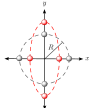
\includegraphics[width=\linewidth]{Efecto-GW-3}
        \caption{Oscilación inducida por una onda gravitacional con polarización $+$ ``apretando" \ el círculo a lo largo del eje $y$.}
        \label{fig:Efecto-GW-3}
    \end{subfigure}\hskip 1em%
    \begin{subfigure}[t]{0.4\textwidth}
        \centering
        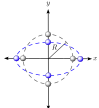
\includegraphics[width=\linewidth]{Efecto-GW-4}
        \caption{Oscilación inducida por una onda gravitacional con polarización $+$ ``estirando" \ el círculo a lo largo del eje $x$.}
        \label{fig:Efecto-GW-4}
    \end{subfigure}
\end{figure}

El cambio de la distancia $L(\varphi)$ es
\begin{equation}
\delta L = L - L_0 \approx R\left[1 - \frac{h_{+}}{2} \cos(\omega t_{0} - kz - \varphi_{+} ) \right] \cos(2\varphi) - R \sim \frac{R h_{+}}{2},
\end{equation}
es decir,
\begin{shaded}
\begin{equation}
\frac{\delta L}{L_0} \sim h.
\end{equation}
\end{shaded}

Los detectores de ondas gravitacionales interferométricos actuales alcanzan una sensibilidad que permite detectar amplitudes hasta de $h \sim 10^{-20}$. Por ejemplo, el proyecto LIGO. consta de un interferómetro de $4 \,[\text{km}]$, de modo que puede detectar fluctuaciones de distancia
\begin{equation}
\delta L \sim L_0 h = (4 \times 10^{3} \,[\text{m}]) \cdot (10^{-20}) \sim 10^{-17} \,[\text{m}],
\end{equation}
es decir, más pequeñas que un núcleo atómico ($\sim 1 \,[\text{fm}] = 10^{-15}\,[\text{m}] $).
\end{document}
